\documentclass{IEEEtran}
\usepackage[utf8]{inputenc}
\usepackage{graphicx}
\usepackage{subcaption}
\usepackage{url}
\usepackage{amsmath}
\usepackage{wrapfig, framed, caption}

%Useful links
%G-Power downloads
    %https://www.psychologie.hhu.de/arbeitsgruppen/allgemeine-psychologie-und-arbeitspsychologie/gpower
    %https://learningspace.falmouth.ac.uk/mod/resource/view.php?id=245797

%\title{Evaluating the use of Adaptive AI to Build Player-Companion Collaboration} 
%Evaluating Collaboration With AI NPCs to Build Player-Companion Relationships
\title{Does the use of adaptive AI help to build player-companion collaboration?}
\author{Andrew J. Scott}  
\date{September 2022}

\begin{document}
	\maketitle
	\pagenumbering{arabic}

%Careful with the use of I in text, even in abstract. Sometimes we is used, but try to avoid it if possible
%This proposal demonstrates...

\begin{abstract}
In this dissertation, I demonstrate the use of adaptive AI for companion characters. The adaptive AI will respond to player actions so it can collaborate with them better. I am testing to see if this adaption helps to make the companion character perceived as more collaborative by the player.
\end{abstract}

 \begin{IEEEkeywords}
Artificial Intelligence, AI, Synergy, Collaboration, Cooperation, Companion, NPC, Adaptive, Game.
\end{IEEEkeywords}

\section{Introduction}
\label{Intro}

%Rephrase citations to make it clearer I am talking about the talks/chapters, as it looks like I am referencing the games themselves
I am planning to develop an AI companion, similar to Atreus in \textit{God of War} \cite{GDCAtreus} or Ellie from \textit{The Last of Us} \cite{GAIP2EllieAI}, which will aid the player in combat. The focus of this project would be on using agent modelling, outlined in section \ref{AgentModelling}, to make an adaptive AI that determines how the companion can best assist the player without requiring any explicit commands from them.

I am planning on building upon these companion characters by focusing on the sense of collaboration between them and the player. There are five core design pillars that I’m considering:

\label{CoreDesign}
\begin{itemize}
	\item \textbf{Enhances Agency} - The AI will have to balance multiple duties, such as helping the player stay safe, attacking other enemies so they do not get overwhelmed and maintaining their own safety \cite{CoupledEmpowermentMaximisation, tremblay2013adaptive}.
	\item \textbf{Doesn't Overshadow} - I plan to ensure that this AI does not overshadow the player \cite{CoupledEmpowermentMaximisation, DesignDocAIAllies} by making their behaviours mostly supportive.
	\item \textbf{No Explicit Commands} - I plan to enable collaboration without explicit commands, as this ruins the companion's own agency \cite{EGXCharacterDeathGuildWars}.
	\item \textbf{Simple Behaviours} - I will keep the combat actions simple, both for the player and companion actions. This reduces scope and allows the AI to be incorporated in other action games easier. This is standard in industry \cite{GMTGoodAI, GDCLessIsMore, GDCSimplestAITrick}.
	\item \textbf{Low Maintenance} - While the player should be able to notice the AI, they should not need to rely on them for specific behaviours or completely change their playstyle to get the AI to be helpful.
\end{itemize}

\section{Background}
\label{Background}

Background, motivations, etc.

\section{Related Work}
\label{RelatedWork}

%Be careful when making claims like this
Research in 2010 highlights the lack of AI research in games \cite{RealTimeAICritique2010}. Additionally, \textit{The Elder Scrolls V: Skyrim}, released in 2011, is criticised for their AI companions \cite{tremblay2013adaptive}, specifically the poor pathfinding behaviour, which can result in companions moving in front of the player when they are trying to attack.

%Cite review and analysis sources for companions

%Expand on the sources in the following sentence to distinguish them, rather than talking about them generally: Specifically looking at companion characters, there is a lot of research on implementing adaptive behaviour \cite{tremblay2013adaptive, CompanionBotsFPS2019, GeneratingCollabBehaviourPlanRecognition2016}
Since then, there has been a lot of improvements in AI research. Specifically looking at companion characters, there is a lot of research on implementing adaptive behaviour \cite{tremblay2013adaptive, CompanionBotsFPS2019, GeneratingCollabBehaviourPlanRecognition2016}. In industry, games like \textit{God of War 2018}, \textit{The Last of Us} and \textit{Bioshock Infinite} are renowned for their AI companions \cite{PlayDontShow} (cite more reviews and analyses). All three of the studios behind these games have developed AI techniques to fine-tune behaviour \cite{GDCAtreus, GAIP2EllieAI, GDCElizabeth, AIGamesBioshockAI}.

\subsection{Responsive Behaviour}
\label{Responsive Behaviour}

Atreus in \textit{God of War 2018} is a good example of synergistic AI, as he will help the player land slow attacks and will extend enemy vulnerability by shooting them with arrows \cite{GDCAtreus}. For example, when the player launches an enemy into the air, Atreus will shoot them and keep them there. There is also a lot of emphasis on his character development over the course of the game, which is reflected in his behaviour. At the start of the game, he only takes actions when commanded, and learns to be more automated towards the middle of the game. Later, he becomes brash, so he starts to outright ignore the players’ commands, and performs actions that would otherwise only occur when commanded, like his special runic abilities. These changes in his AI help to tie the narrative into gameplay and make him seem like a real character, which helps to allow the player to bond with Atreus. These changes are also noticeable when the player is separated from Atreus, which helps the players realise how much they rely on him.

\begin{figure}
  \centering
  \includegraphics[width=\linewidth]{Images/TLOUPathfinding.png}
  
\caption{Pathfinding diagram in \textit{The Last of Us}}
\label{fig:TLOUPathfinding}
\end{figure}

\subsection{AI Movement}
\label{Movement}

%The Skyrim pathfinding point was made earlier, consider removing
%Consider talking about the theatre techniques used in Bioshock: Infinite
Pathfinding is an important aspect of AI companions. The AI needs to be close to the player so that it is not forgotten \cite{GAIP2EllieAI}, but also not too close that it gets in their way and obstructs them \cite{CoupledEmpowermentMaximisation}. An example of poor AI pathfinding is in \textit{Skyrim} \cite{tremblay2013adaptive}, where the AI will move in front of the player when they are aiming and generally get in their way when moving. Naughty Dog addressed these issues in \textit{The Last of Us} with pathfinding tools, shown in figure \ref{fig:TLOUPathfinding}, that keeps companions close to the player, but not in the way \cite{GAIP2EllieAI}. Ellie will also move out of the way if the player moves into her personal space. Vocal barks are used in such moments to add character, and while it is a good practice to use voice acting to help make the player aware of the agent’s actions, and make them feel more real \cite{GMTGoodAI}, they are not suitable for games with lower budgets.

\begin{figure}
  \centering
  
  \begin{subfigure}[a]{\linewidth}
  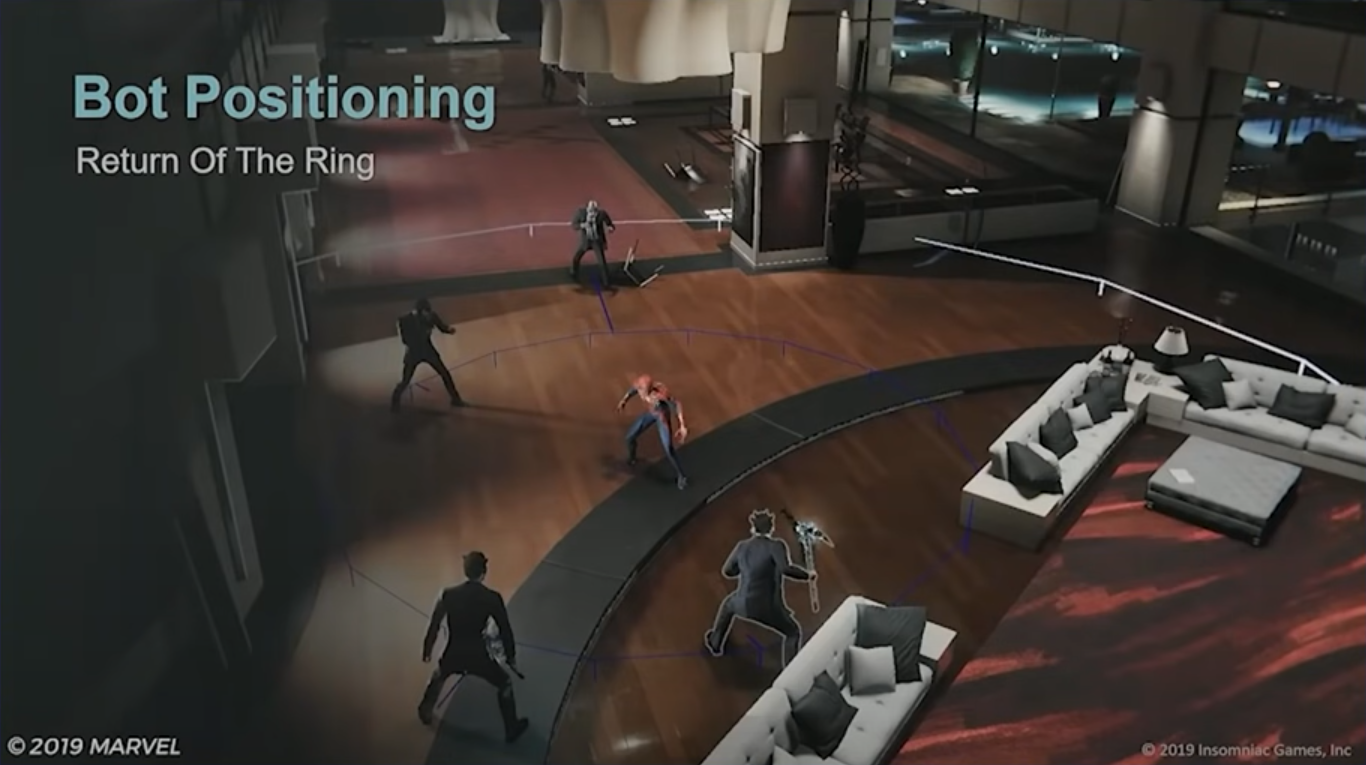
\includegraphics[width=\linewidth]{Images/SpidermanKungFuCircle.png}
  \end{subfigure}
  
  \begin{subfigure}[b]{\linewidth}
  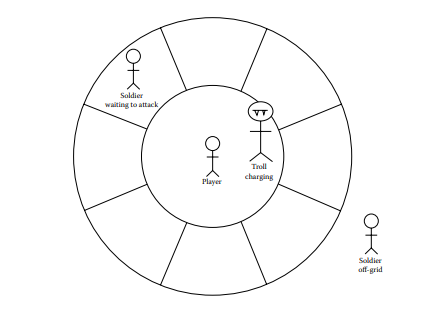
\includegraphics[width=\linewidth]{Images/KOARKungFuCircle.png}
  \end{subfigure}
  
  \caption{Demonstration of Kung-Fu Circles in (a) \textit{Marvel's Spiderman} and (b) \textit{Kingdoms of Amalur: Reckoning}}
  \label{fig:KungFuCircle}
\end{figure}

Many action games, such as \textit{Marvel's Spiderman} and \textit{Kingdoms of Amalur: Reckoning}, use a technique known as the Kung-Fu Circle to manage the positioning of multiple agents \cite{GAIPKungFuCircle, GDCSpiderman}, shown in figure \ref{fig:KungFuCircle}. An AI manager handles the positioning of enemies in this circle and manages when they can attack. While this technique is intended to manage multiple enemies in action games, I can also use it to determine where the AI companion could be placed.

\subsection{Animations, Bespoke Behaviours and Call-outs}
\label{ABC}

A lot of industry practice with developing AI for companion characters is to use bespoke behaviour, detailed animations and vocal call-outs to give personality and character \cite{GAIP2EllieAI, GMTGoodAI, GAIPOReactions}. In particular, Irrational Games created a smart terrain system for \textit{Bioshock Infinite} that allows Elizabeth to interact with the environment \cite{GDCElizabeth, AIGamesBioshockAI}, shown in figure \ref{fig:BioshockSmartTerrain}. A lot of these finishing touches are a key part of making the companion feel more believable, allowing the player to empathise and engage with them more. It also helps to communicate NPC actions, so the player understands that they are actually making choices, otherwise they can miss the intelligence of the AI \cite{GMTGoodAI}.

Instead of focusing on animation and voice lines, I am planning to focus on using adaptive AI to improve the sense of collaboration between them. The intent of this would be to improve player-companion relationships in games with lower budgets and to maximise them in games that can have animations and voice acting. To do this, I will implement AI techniques that allow a companion NPC to adapt to player actions to collaborate with them better.

\begin{figure}
  \centering
  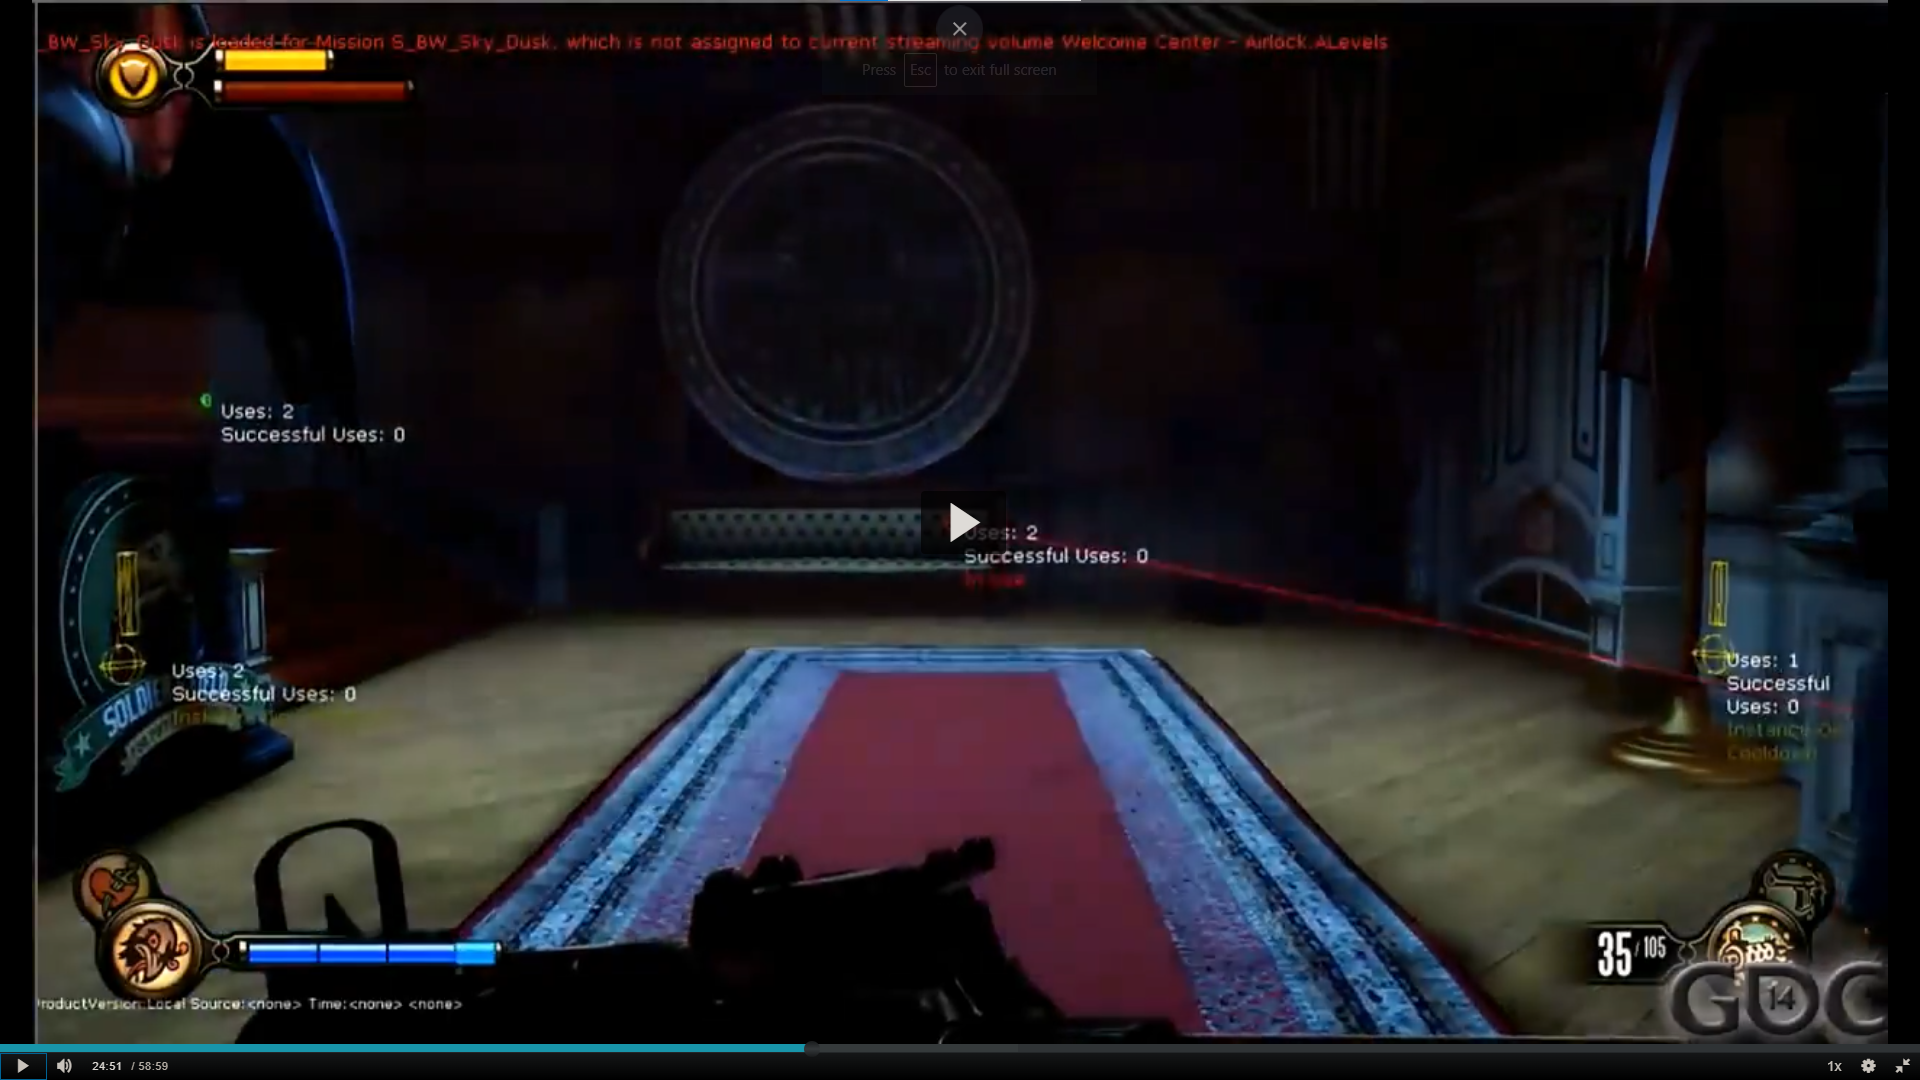
\includegraphics[width=\linewidth]{Images/BioshockSmartTerrain.png}
  
\caption{Smart Terrain showcase in \textit{Bioshock: Infinite}}
\label{fig:BioshockSmartTerrain}
\end{figure}

\subsection{Collaboration Without Communication}
\label{Communication}

My core design, detailed in Section \ref{CoreDesign}, is that the player cannot explicitly command the companion. As a result, the AI needs to determine how to collaborate with the player without communication. The following methods are some ways in which an AI can collaborate with other agents without communication.

\subsubsection{Plan Recognition}
\label{PlanRecognition}

Plan recognition is a useful technique for agents that need to collaborate with other agents, including players, without requiring explicit commands or communication \cite{GeneratingCollabBehaviourPlanRecognition2016, PandemicPlanRecognition2021}. Agents that use plan recognition observe the actions taken by another entity in order to determine their goals. Once an entity’s goal has been identified, the plan recognition agent will devise actions that can aid them in achieving their goals \cite{GeneratingCollabBehaviourPlanRecognition2016}. A common use for this technique is in RTS games \cite{PlayerAdaptiveRTSAI2007} as agents use observed behaviour to determine their allies' or opponents' plans.

Plan recognition agents can also be used for board games where multiple agents must work together for a common goal but have no or limited communication with each other \cite{PandemicPlanRecognition2021}. Agents must determine their their team member's plans based on their actions and determine what they can do to better support them.

Implementing a plan recognition agent in an action game requires a more complex combat system. This type of agent could be useful in an action game with combos, where the AI will be required to determine which attack in the combo the player plans to use, and will plan attacks that collaborate well with them. For example, if the player is building up to a slow attack, they will interrupt enemies from hitting the player and will prevent the target from escaping. If the player is planning a large AOE attack, they will try to stagger enemies into the effect and keep them there. This will ideally make the AI seem intelligent and build collaboration while also appearing to give the AI more agency as it does not respond to player actions directly.

However, these behaviours would be much more reliable with bespoke behaviours, especially since the actions taken by the agent in both examples are quite similar. Using a plan recognition agent in an action game would require the combat system to be complex enough that the agent needs to use unique actions for various plans, which breaks one of my core design pillars outlined in section \ref{CoreDesign}. Looking at Atreus \textit{God of War 2018}, analysed in section \ref{RelatedWork}, all the actions Atreus uses are very similar, but it’s the timing that is important \cite{GDCAtreus}.

\subsubsection{Agent Modelling}
\label{AgentModelling}

%Need more info in this section
Agent modelling is another technique for agents that need to take actions based on another entity. Similar to plan recognition, an agent modelling AI observes actions and acts upon them \cite{yannakakis2013playermodelling}. However, instead of using the actions to determine an entity’s goals, it constructs a model of the entity, which is used to define more overall strategies. This model is then used to determine the agent's actions in response. Like plan recognition, agent modelling techniques tend to be used for AI in RTS games \cite{OpponentModellingRTS2007, bakkes2009opponentmodelling}. It is also used in similar board games like \textit{Hanabi} \cite{EvaluatingHanabiAgents}.

\subsubsection{Other Methods}
\label{OtherConsiderations}

%Need more info in this section
Theory of Mind methods \cite{TheoryOfMind2013, von2017mindsofmany}.

%Eger source also has works on Hanabi and Pandemic, consider restructuring to include Pandemic and Hanabi research in 1 secion to show a line of research
Another AI technique for \textit{Hanabi} is to use time to communicate between agents \cite{WaitASecond2019}. While this is effective for collaboration between AI agents, this method is not reliable for player-AI collaboration.

\section{Proposed Research}
\label{ProposedResearch}

\subsection{Research Question}
\label{ResearchQuestion}

Research question here

\subsection{Hypothesis}
\label{Hypotheses}
%Need more info in this section
My hypothesis is that participants that are given the adaptive AI will rate their companion as more collaborative as those without. This means that adaptability has a positive influence on player’s perception of collaboration.

The null hypothesis is that participants that there will be no difference in the ratings for each of the AI companions. This means that adaptability has no discernible effect on player’s perception of collaboration.

\section{Research Method}
\label{ResearchMethod}

\subsection{Philosophical Position}
\label{PhilosophicalPosition}

Philosophy

\subsection{Experimental Design}
\label{ExperimentalDesign}

%Need more info in this section

%Might be best to have each participant play both as they could be skewed by personal biases so the baseline needs to be established randomise the order

%G-Power video explanation: https://web.microsoftstream.com/video/d1ec1c56-bb97-4592-ae4e-1c973e3fee20?referrer=https:%2F%2Flearningspace.falmouth.ac.uk%2F

I plan to set up two versions of an action game with a companion character. The first version will feature a simple AI which will simply attack the closest target with random attacks and use basic path-finding to keep close to the player when not attacking. The second version will feature an adaptive AI, which will determine target's based on the player actions and will choose attacks that support the player's intentions better.

I plan to collect opinions on the AI using structured observations and questionnaires. I plan to give each participant one of the versions to play through and will give them a questionnaire which should help to evaluate them. Some of the questions would start out establishing the participant's prior experience with games and what kind of games they like, and will then move onto the specifics in the AI.

\subsection{Data Management Plan}
\label{DataManagementPlan}

I plan to collect opinions on the AI using structured observations and questionnaires. I plan to give each participant one of the versions to play through and will give them a questionnaire which should help to evaluate them. Some of the questions would start out establishing the participant's prior experience with games and what kind of games they like, and will then move onto the specifics in the AI.

%Highlight that I am focusing on perception of AI
%More info on the types of questions used
%Double check use of et al
Most of the questions will use a Likert scale to distil responses into quantitative data and will include questions on how likeable, intelligent, collaborative, etc. the player thought they were. I am planning to use a similar approach to the one used by Z. Ashktorab et al \cite{SocialPerceptions2020} as I am also looking to gather opinions on an AI. I will have qualitative questions that allow participants to put sentence answers so they can give more specific thoughts. This will also help to determine if there are any bugs that caused one AI to not work as intended.

\subsection{Ethical Considerations}
\label{EthicalConsiderations}

Ethical considerations here

\section{Expected Outcomes}
\label{ExpectedOutcomes}

Expected outcomes here
 
\section*{Acknowledgments}

%Joe, Michael and Liz
%Falmouth Uni
Acknowledgements here

%Careful with some sources, make sure they are all correct and careful with videos
%Specify that some are conferences
\bibliographystyle{IEEEtran}
\bibliography{bibliography} 

\end{document}